\chapter{Standard di Telefonia Mobile \emph{LTE}}
\label{cap:lte}
\begin{figure}[h]
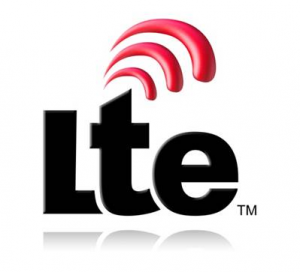
\includegraphics[scale=0.5]{Immagini/lte}
\centering 
\end{figure}

Il sistema \ac{LTE} è un esempio importante di tecnologia radiomobile di quarta generazione (\emph{4G}) in grado di offrire servizi 
a larga banda. Se l'attuale generazione di reti di telecomunicazione mobile è nota come 3G, \ac{LTE} è, impropriamente, commercializzato 
come \emph{4G} (Fig. \ref{img:lte4g}).

\begin{figure}
 \centering
 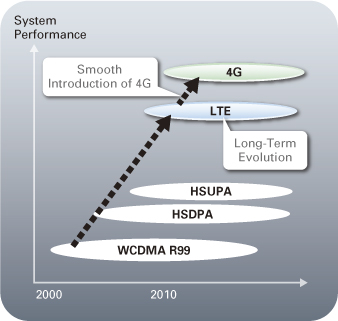
\includegraphics[scale=0.5]{Immagini/lte4g}
 \caption{L'evoluzione delle tecnologie mobili.}
 \label{img:lte4g}
\end{figure}

Secondo \ac{3GPP}, in \ac{LTE} sono identificati una serie di requisiti ad alto livello;
\begin{itemize}
 \item Riduzione dei costi per bit.
 \item Fornitura di più servizi a costi inferiori e con migliore esperienza utente.
 \item Flessibilità nell'utilizzo di bande frequenza nuove o esistenti.
 \item Architettura semplificata.
 \item Consentire un ragionevole consumo energetico del terminale.
\end{itemize}

Nonostante ci sia una sostanziale differenza rispetto ai suoi predecessori, \ac{LTE} è considerato un'evoluzione dello standard \emph{3G},
Nella tabella \ref{tab:confronto}, sono mostrate le principali differenze con le tecnologie precedenti:

 \begin{table}[h]\footnotesize
  \caption{Confronto tra le attuali e future tecnologie mobili}
  \label{tab:confronto}
  \begin{tabularx}{\textwidth}{XXXXXX}
    \toprule
      & WCDMA (UMTS) & HSDPA & HSDPA+ & LTE & LTE Advanced \\
    \midrule
      Max Downlink Speed & 384 kb/s & 14 Mb/s & 42 Mb/s & 326,4 Mb/s & 3,3 Gb/s \\
      Max Uplink Speed & 128 kb/s & 5,7 Mb/s & 11 Mb/s & 86,4 Mb/s & Sconosciuto \\
      Latency round trip time (ms) & 150 & 100 & 50 & ~ 10 & Sconosciuto \\
      3GPP Releases & Rel 99/4 & Rel 5/6 & Rel 7 & Rel 8 & Rel 10 \\
      Access methodology & CDMA & CDMA & CDMA & OFDMA / SC-FDMA & OFDMA Ibrido / SC-FDMA \\
    \bottomrule
    \end{tabularx}
  \end{table}

I motivi che hanno spinto a questa nuova tecnologia sono stati vari:
\begin{itemize}
 \item Necessità di garantire la continuità della competitività del sistema 3G per il futuro.
 \item Domanda degli utenti per velocità di trasferimento dati più elevate e qualità del servizio.
 \item Sistema ottimizzato di commutazione a pacchetto.
 \item Continua richiesta di riduzione dei costi (CAPEX e OPEX).
 \item Complessità bassa.
 \item Evitare un'inutile frammentazione delle tecnologie per la banda di funzionamento.
\end{itemize}

\section{Caratteristiche}
\label{sub:caratteristiche}
Lo standard \ac{LTE} affronta l'aggiornamento dal \emph{3G UMTS} verso quello che sarà chiamato standard comunicazione mobile di quarta 
generazione \emph{4G}. La maggior parte del lavoro mira a semplificare l'architettura del sistema, per esempio per le 
chiamate vocali, come discusso nel paragrafo \ref{sub:voice}, da una rete a commutazione a pacchetto (per i dati) e a commutazione a 
circuito (per le chiamate vocali) dell'attuale tecnologia \emph{UMTS}, verso un architettura completamente basata su \emph{IP}. \\
L'interfaccia fisica di trasmissione radio utilizzata in \ac{LTE} è detta \emph{E-UTRA}, le sue principali caratteristiche sono:
\begin{itemize}
 \item Velocità di download di picco di $299 Mbit/s$ e upload fino a $75.4 Mbit/s$.
 \item Latenze ridotte (inferiori ai 100 ms per il passaggio dallo stato idle allo stato active, ed in-
  feriori ai 5 ms per piccoli pacchetti IP)
 \item Migliorato il supporto per la mobilità, esemplificato da supporto per i terminali in movimento fino a $350 km/h$ o $500 km/h$ 
  a seconda della banda di frequenza.
 \item \emph{OFDMA} per il downlink\footnotemark[1] e \emph{SC-FDMA} per l'uplink\footnotemark[2].
 \item Supporto per i sistemi di comunicazione \ac{FDD} e \ac{TDD} e half-duplex \ac{FDD} con la stessa tecnologia di accesso radio.
 \item Supporto per dimensioni delle celle variabili: da decine di metri di raggio (femto e picocelle) fino a $100 km$ di raggio (macrocelle).
  Le bande di frequenza più basse sono utilizzate nelle zone rurali, con dimensioni cellulari da $5 km$ con prestazioni ottimali, fino a $100 
  km$ con prestazioni accettabili. Nelle aree urbane e urbane, bande di frequenza più elevate (ad esempio $2,6 GHz$ in EU) sono usate per 
  sostenere banda larga ad alta velocità mobile. In questo caso, le dimensioni delle celle può essere $1 km$ o anche meno.
 \item Supporto per almeno 200 clienti attivi per cella da $5 MHz$.
 \item Supporto per l'inter-operabilità e la coesistenza con tecnologie precedenti: gli utenti possono avviare una chiamata o il 
  trasferimento di dati in una zona con uno standard \ac{LTE}, e, se la copertura non è disponibile, continuare l'operazione senza alcuna 
  azione da parte loro passando a tecnologi precedenti come \emph{GSM / GPRS} o \emph{W-CDMA} o anche le reti \emph{UMTS}.
 \item Elevata efficienza spettale (numero di bit/s trasmessi per ogni Hz impiegato) 3 volte superiore alla più evoluta versione 
  dell'\emph{UMTS}, ovvero l'\emph{HSPA}.
\end{itemize}
\footnotetext[1]{Collegamento tra una stazione base e la stazione mobile ad essa associata}
\footnotetext[2]{Percorso dei dati da un telefono cellulare alla centrale}

 \subsection{Standard e frequenze}
 Nell'Unione Europea lo standard \ac{LTE} lavora sulle seguenti bande di frequenza:
 \begin{description}
  \item[800 MHz] in Italia dal 2013 sarà possibile sfruttare questa banda non appena sarà completo il passaggio al digitale terrestre
  \item[900 MHz] questa banda attualmente imegnata dal \emph{GSM} attraverso un \emph{refarming dello spettro} sarà disponibile per 
		  l'\ac{LTE}
  \item[1800 MHz] entro il 2012 saranno disponibili alcuni canali occupati dal GSM
  \item[2600 MHz] frequenze libere tranne che in alcune zone utilizzate dal ministero della difesa o da radar
 \end{description}
 
\subsubsection{OFDMA}
Uno degli elementi chiave di \ac{LTE} è l'uso di \ac{OFDM} per trasportare il segnale e gli schemi di accesso associati: \emph{OFDMA} 
(Orthogonal Frequency Division Multiple Access) e \emph{SC-FDMA} (Single Carrier Frequency Division Multiple Access). \\
\ac{OFDM} è già utilizzato in altri sistemi come \emph{WLAN} e \emph{WiMAX} per l'audio e il video \emph{broadcasting}; l'\ac{OFDM} ha
molti vantaggi tra cui la robustezza al \emph{fading} multiplo e alle interferenze.
\ac{OFDM} è un tipo di trasmissione che usa un gran numero di portanti vicini tra loro, modulati con basso \emph{symbol rate}. Normalmente 
ci si aspetterebbe che questi segnali interferiscano l'uno con l'altro, ma facendo in modo che siano ortogonali tra loro non c'è 
interferenza reciproca. Ciò si ottiene spaziando le portanti del reciproco del periodo di simbolo. \\
Questo significa che quando i segnali sono demodulati avranno un numero intero di cicli nel periodo di simbolo e il loro contributo si 
somma a zero, quindi non vi è alcun contributo di interferenza. 
I dati da trasmettere sono suddivisi su tutte le portanti, e attraverso l'utilizzo di tecniche di correzione di errore, se alcune 
frequenze portanti vengono perse a causa di effetti di \emph{fading} multiplo, i dati possono essere ricostruiti.  \\
Inoltre avendo dati trasmesso ad un basso \emph{symbol rate} attraverso tutte le portanti significa che gli effetti di riflessione e 
interferenza intersimbolica possono essere superati. Significa anche che reti a singola frequenza, in cui tutti i trasmettitori possono
trasmettere sul canale stesso, possono essere implementate.

\begin{figure}
 \centering
 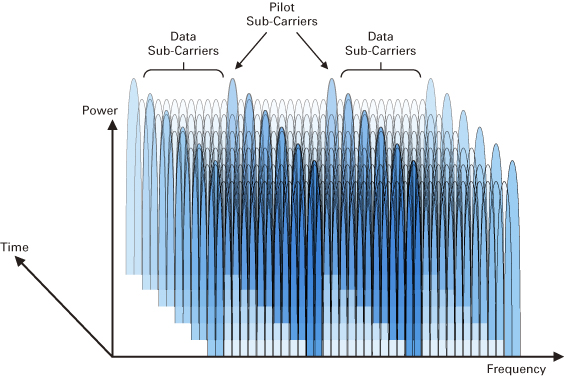
\includegraphics[scale=0.5]{Immagini/ofdma}
 \caption{OFDMA.}
 \label{img:ofdma}
\end{figure}
 
% \subsubsection{MIMO}
% L'acronimo \emph{MIMO} vuol dire \emph{Multiple-Input and Multiple-Output}, cioè entrate multiple ed uscite multiple, in \ac{LTE} sta ad 
% indicare la possibilità di un utilizzo di antenne multiple sia per il mittente per il ricevente per migliorare le prestazioni della
% comunicazione, come mostrato nella fiugra \ref{img:mimo}. \\
% La tecnologia \emph{MIMO} ha attirato l'attenzione nelle comunicazioni wireless, perché offre un aumento significativo del 
% \emph{throughput}, la capacità di trasmissione effettivamente utilizzata, senza ulteriore larghezza di banda o aumento di potenza di 
% trasmissione.
% Questi risultati possono essere raggiunti diffondendo la stessa potenza totale sulle antenne per ottenere una matrice di guadagno (Fig.
% \ref{img:mimomatrix} che migliora l'efficienza spettrale (più bit per secondo per hertz di banda) o per ottenere un guadagno che 
% migliora l'affidabilità collegamento (fading ridotto). 
% A causa di queste proprietà, \emph{MIMO} è una parte importante delle moderne tecnologie di comunicazione wireless come 
% \emph{IEEE 802.11n (Wi-Fi)}, \emph{4G}, \emph{WiMAX} e \emph{HSPA +}, oltre che, ovviamente, \ac{LTE}.
% 
% \begin{figure}[!h]
% 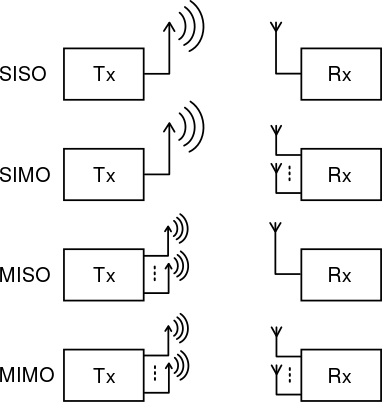
\includegraphics[scale=0.5]{Immagini/mimo}
% \centering 
% \caption{Configurazioni SISO, SIMO, MISO e MIMO, l'ingresso e l'uscita si riferiscono al canale radio che porta il segnale, non alle 
% antenne che hanno i dispositivi.}
% \label{img:mimo}
% \end{figure}
% 
% \begin{figure}[!h]
% 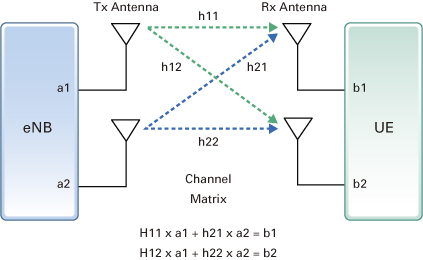
\includegraphics[scale=0.5]{Immagini/mimomatrix}
% \centering 
% \caption{Matrice di guadagno $2 \times 2$.}
% \label{img:mimomatrix}
% \end{figure}

 \subsection{Architettura di rete}
 La rete di accesso di \ac{LTE}, detta anche \ac{E-UTRA}, è costituita da un unico elemento, il cosiddetto \ac{eNB}.
 In \ac{LTE}, al contrario che nelle precedenti tecnologie, è possibile semplificare l'architettura di rete nel solo \ac{eNB} (Fig. \ref{img:enb}),
 in quanto tutti dati, anche quelli voce, viaggiano su protocolli a pacchetto; il grande vantaggio, inoltre, è che i nodi sono 
 interconnessi tramite interfacce standardizzate in modo da garantire la compatibilità con le tecnologie precedenti. \\
 Gli \ac{eNB} sono interconnessi tramite le interfacce \emph{X2}. Si presume che esista sempre un'interfaccia X2 tra gli 
 \ac{eNB} che devono comunicare tra loro, ad esempio, per il supporto del trasferimento dell'\ac{UE} nello stato \emph{active}. 
 Gli \ac{eNB} sono collegati anche mediante l'interfaccia \emph{S1} alla \emph{EPC} (Evolved Packet Core). L'interfaccia \emph{S1} 
 supporta una relazione molti-a-molti tra \emph{aGW} e \ac{eNB}.
 
 \begin{figure}[!h]
 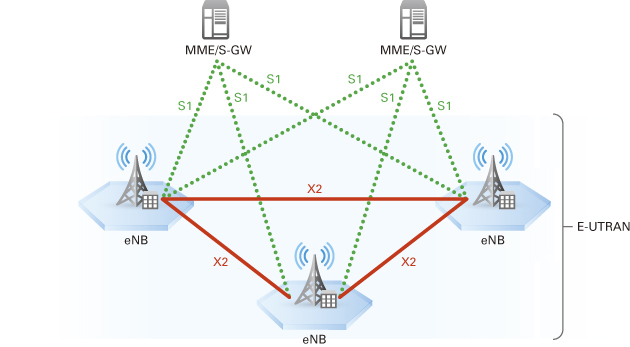
\includegraphics[scale=0.5]{Immagini/enb}
 \centering 
 \caption{Architettura di rete \ac{LTE}}
 \label{img:enb}
 \end{figure}
 
 \subsubsection{User Equipment}
 Il dispositivo \ac{LTE} è detto \ac{UE} come già avveniva con l'\emph{UMTS}, questo termine sta proprio ad evidenziare l'avanzato apparato
 tecnologico che si porta dietro l'utente. L'\ac{UE} è costituito da due parti: il \emph{Mobile Equipment}, cioè l'hardware che costituisce
 il dispositivo e il software ch permette la connessione alla rete, e la \emph{Universal Subscriber Identity Module}, il circuito integrato
 che contiene le informazioni legate all'utente, alla rete e ai servizi supportati.
  
\subsection{Quality of Service}
\label{sec:qos}
L'\ac{LTE} fornisce diverse qualità di servizio \ac{QoS}, ogni flusso informativo è associato ad una specifica classe di \ac{QoS}, i 
livelli di \ac{QoS} offerti sono due:
\begin{description}
 \item[GBR] (minimum Guaranteed Bit Rate): questo tipo di servizio offre risorse dedicate per tutta la durata della trasmissione, alti
 data rate, ritardi contenuti e  tassi d'errore contenuti;  l'utilizzo principale è quello voce, come le chiamate vocali o il \emph{VoIP}.
 \item[Non-GBR]: questo servizio sono utilizzati per applicazioni che non richiedono bitrate particolarmente elevati, come il web browsing
 o i trasferimenti FTP.
\end{description}

 \subsection{Mobilità e Handover}
 Un terminale all'interno di \ac{LTE} può trovarsi in tre stati: \emph{detached}, \emph{active}, \emph{idle}.
 \begin{figure}[!h]
 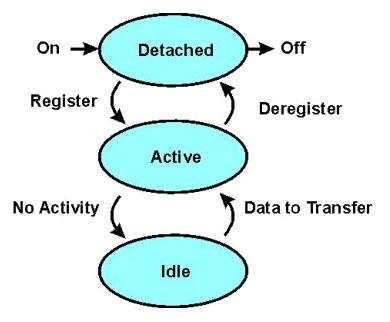
\includegraphics[scale=0.5]{Immagini/ltestatus}
 \centering 
 \caption{Stati di un dispositivo mobile \emph{LTE}.}
 \end{figure}
 Non appena il dispositivo viene acceso, esso si trova nello stato \emph{detached}: è attivo ma non è ancora connesso alla rete. Questa
 è la fase dell'instaurazione della connessione, l'utente è registrato presso l'eNB e passa nello stato \emph{active}. Infine, se l'utente
 non trasmette o riceve per un determinato tempo passa nello stato \emph{idle}. \\
 La posizione di un utente è nota alla rete attraverso la granularità di una \ac{TA}, l'\ac{UE} è memorizzato in un'area geografica, che
 potrebbe essere una \ac{TA} o un elenco di \ac{TA}; il nodo di controllo avvia il \emph{paging} per ciascun \ac{eNB} con celle 
 appartenenti all'\ac{UE}, l'utente passa da \emph{idle} a \emph{active} e può ricevere una chiamata. Ogni \ac{eNB} può contenere celle 
 appartenenti a diverse \ac{TA}, mentre ogni cella può appartenere ad una sola \ac{TA}. \\
 Con riferimento alla figura \ref{img:enb} in \ac{LTE} esistono due tipi di \emph{Handover}, essi si distinguono in base all'interfaccia su
 cui si muove l'\ac{UE}, \emph{X2} o \emph{S1}:
 \begin{description}
  \item[X2] Si riferisce al caso in cui l'utente si muove tra due \ac{eNB}, sempre gestiti dallo stesso \emph{aGW}, cioè all'interno della
  stessa \ac{TA}. L'\emph{handover} avviene sull'interfaccia \emph{X2} tra l'\ac{eNB} su cui è attualmente agganciato (\emph{serving)} e
  il prossimo \ac{eNB} che servirà l'\ac{UE} (\emph{target}), solo questi due nodi sono coinvolti, di conseguenza l'\emph{handover} è
  rapido e richiede poche risorse. Al termine della procedura l'\emph{aGW} è avvisato del cambio di posizione. \\
  Inoltre a seconda delle esigenze dell'\ac{UE} possono avvenire due tipi di \emph{handover}, i quali, ovviamente, sono strettamente legati
  al \ac{QoS} (paragrafo \ref{sec:qos}):
  \begin{itemize}
   \item seamless: questo tipo di \emph{handover} è particolarmente sensibile ai ritardi, quindi è utilizzato nel caso in cui l'\ac{UE} 
   abbia bisogno di servizi \emph{real-time} come, ad esempio, una chiamata vocale.
   \item lossless: in questo tipo di \emph{handover}, invece, lo scopo principale è mantenere un basso tasso di errori e ridurre le perdite
   di pacchetti.
  \end{itemize}

  \item[S1] In questo caso l'\ac{UE} si muove da una \ac{TA} ad un'altra. Questo tipo di \emph{handover} in \ac{LTE} è di tipo \emph{hard},
  la connessione è brevemente interrotta durante il passaggio da un \ac{eNB} ad un altro, il motivo principale di questa interruzione è
  l'assenza di un nodo di controllo che gestisca il traffico di segnalazione. Di conseguenza la rete è semplificata ad esempio rispetto a
  quella \emph{UMTS}.
 \end{description}

 
 
 \subsection{Chiamate vocali}
 \label{sub:voice}
Lo standard \ac{LTE} supporta solo la \emph{commutazione a pacchetto} nelle sue reti IP. Le chiamate vocali nel \emph{GSM}, \emph{UMTS} e 
\emph{CDMA} sono a circuito, quindi con l'adozione dell'\ac{LTE}, gli operatori telefonici dovrebbero riprogettare la loro rete voce. \\
La differenza principale tra commutazione a pacchetto ed a circuito è che nella prima il flusso di informazione è segmentato in 
\emph{pacchetti} di lunghezza limitata o fissa, come avviene in internet con IP; al contrario, la commutazione a circuito, prevede il 
frazionamento della capacità trasmissiva totale per ogni utente. \\
Per ovviare alla riprogettazione della rete sono state proposte tre soluzioni:
\begin{description}
 \item[VoLTE] (Voice Over \ac{LTE}) Questo tipo di approccio prevede di consegnare la voce come se fosse un flusso all'interno del 
 trasporto dati di \ac{LTE}, in questo modo si aggira la commutazione a pacchetto continuando ad utilizzare quella a circuito.
 \item[CSFB] (Circuit Switched FallBack) In questo approccio, \ac{LTE} fornisce il servizio dati e, quando richiesto il servizio voce, 
 automaticamente ricade nella commutazione a circuito.
 \item[SVLTE] (Simultaneous Voice and \ac{LTE}) Questo approccio, invece, fa coesistere le due tecnologie, adottando l'utilizzo della 
 commutazione a pacchetto per la connessione dati e della commutazione a circuito per le chiamate vocali. 
\end{description}
Un altro tipo di approccio prevederebbe di utilizzare la connessione dati anche per le chiamate voci, come accade per \emph{Google Talk} o
\emph{Skype}, ma è troppo complesso perché costringerebbe ogni utente ad avere una connessione attiva sul proprio dispositivo. \\
La maggior parte dei sostenitori principali di \ac{LTE} hanno preferito e promosso \emph{VoLTE} fin dall'inizio, anche se la soluzione 
migliore sarebbe di passare alla commutazione a pacchetto.
Nei paesi dove questa tecnologia è stata già adottata, nell'attesa della standardizzazione del \emph{VoLTE}, a causa dell'elevata
domanda per le chiamate vocali, è stato necessario introdurre \emph{CSFB} come misura provvisoria. Quindi quando si effettua o si riceve
una chiamata vocale, i telefoni \ac{LTE} ricadranno sulla vecchie reti \emph{2G} e \emph{3G} per la durata della chiamata. \\

\ac{LTE} supporta inoltre le chiamate vocali ad alta qualità (\emph{Voice HD}), per garantire la compatibilità, \ac{3GPP} richiede il codec
\emph{AMR} a banda stretta, ma il codec consigliato per il \emph{VoLTE} è a banda larga, inoltre, nelle reti \ac{3GPP} è obbligatorio il 
campionamento a $16 KHz$. Questo tipo di tecnologia, però, richede che sia il mittente che il destinatario la supportino.


\section{LTE in Italia}
In Italia, il 30 settembre 2011 si è conclusa l'asta per la concessione delle frequenze 4G \ac{LTE} delle tre frequenze disponibili: 
$800$, $1800$ e $2600 Mhz$. Il \date{27 Giugno 2011} nella Gazzetta Ufficiale viene pubblicato il bando per l'assegnazione delle 
frequenze agli operatori mobili italiani:
\begin{itemize}
 \item banda $800 MHz$: \emph{``fino a 6 lotti di frequenze FDD, ciascuno di ampiezza pari a 5 MHz in spettro accoppiato, assegnabili su base 
 nazionale, nominati da 1 a 6.''} \\
 Di questi sei lotti ne sono stati acquistati due per ognuna di queste compagine: \emph{Vodafone Italia}, 
 \emph{Telecom Italia} e \emph{Wind Telecomunicazioni}.
 \item banda $1800 MHz$: \emph{``fino a 3 lotti di frequenze FDD, ciascuno di ampiezza pari a 5 MHz in spettro accoppiato, assegnabili su base 
 nazionale, nominati da 1 a 3.''} \\
 Un blocco a testa è stato aggiudicato da \emph{Vodafone Italia}, \emph{Telecom Italia} e \emph{3 Italia}.
 \item banda $2000 MHz$: \emph{``1 lotto di frequenze TDD di ampiezza pari a 15 MHz, assegnabile su base nazionale, nominato lotto A.''} \\
 Per questo  lotto non è stata effettuata nessuna offerta.
 \item banda $2600 MHz$: \emph{``fino a 12 lotti di frequenze FDD, ciascuno di ampiezza pari a 5 MHz, in spettro accoppiato, assegnabili su base 
 nazionale, nominati da 3 a 14, e 2 lotti di frequenze TDD, ciascuno di ampiezza pari a 15 MHz, assegnabili su base nazionale, nominati 
 lotto B e C, con esclusione delle frequenze 2500-2510 MHz e 2620-2630 MHz nei lotti FDD e delle frequenze 2600-2620 MHz nei lotti TDD.''} \\
 \emph{3 Italia} e \emph{Wind Telecomunicazioni} si aggiudicano quattro blocchi, tre \emph{Vodafone Italia} e \emph{Telecom Italia}.
\end{itemize}

% \section{Sviluppi futuri: LTE-Advanced}
%  L'obiettivo di \ac{3GPP} \ac{LTE} Advanced è quello di raggiungere e superare i requisiti \emph{ITU} (International Telecommunication 
%  Union). \ac{LTE} Advanced dovrebbe essere compatibile e condividere le stesse frequenze dell'attuale \ac{LTE}. \\
%  Uno dei più grandi vantaggi di \ac{LTE} Advanced sarà la capacità di sfruttare avanzate reti topologiche: reti eterogenee ottimizzate con 
%  un mix di macrocelle con nodi a bassa potenza come picocelle e femtocelle. \\
%  \ac{LTE} Advanced introduce anche una multiportante per essere in grado di utilizzare una ultra banda larga, fino a $100 MHz$ di spettro 
%  supportando velocità molto elevate. Nella fase di ricerca che ha portato ad \ac{LTE} Advanced le proposte sono state svariate, esse 
%  possono essere suddivise principalmente in:
%  \begin{itemize}
%   \item Trasmissione e ricezione coordinata (\emph{CoMP}).
%   \item Supporto per il \emph{SU-MIMO} sull'antenna trasmittente dell'\ac{UE}.
%   \item Banda del sistema scalabile superiore a 20 MHz, fino a 100 MHz.
%   \item Flessibilità dello spettro.
%   \item Cognitive radio
%   \item Configurazione e funzionamento di rete automatico e autonomo.
%   \item Maggiore precodifica e rilevazione e successiva correzione degli errori.
%   \item Gestione dell'interferenza e la soppressione.
%   \item Assegnazione della larghezza di banda asimmetrica per ac{FDD}.
%   \item Uplink ibrido con \emph{OFDMA} e \emph{SC-FDMA}.
%   \item Accesso multiplo delle portanti allo spettro.
%  \end{itemize}
  
